\documentclass[12pt]{article}
\usepackage{geometry}                % See geometry.pdf to learn the layout options. There are lots.
\geometry{letterpaper}                   % ... or a4paper or a5paper or ... 
%\geometry{landscape}                % Activate for for rotated page geometry
\usepackage[parfill]{parskip}    % Activate to begin paragraphs with an empty line rather than an indent
\usepackage{daves,fancyhdr,natbib,graphicx,dcolumn,amsmath,lastpage,url}
\usepackage{amsmath,amssymb,epstopdf,longtable}
\DeclareGraphicsRule{.tif}{png}{.png}{`convert #1 `dirname #1`/`basename #1 .tif`.png}
\pagestyle{fancy}
\lhead{CE 3354 -- Engineering Hydrology}
\rhead{FALL 2024}
\lfoot{ES7}
\cfoot{}
\rfoot{Page \thepage\ of \pageref{LastPage}}
\renewcommand\headrulewidth{0pt}



\begin{document}
\begin{center}
{\textbf{{ CE 3354 Engineering Hydrology} \\ {Exercise Set 7}}}
\end{center}

 \section*{\small{Exercises}}
Figure \ref{fig:RockyRun} is a Google-Earth image of some watershed.  The red boundary defines the watershed;  The distance on the image from Rain Gage R-1 to the Rocky Run Branch Gage is 1,500 feet.

\begin{figure}[h!] %  figure placement: here, top, bottom, or page
   \centering
   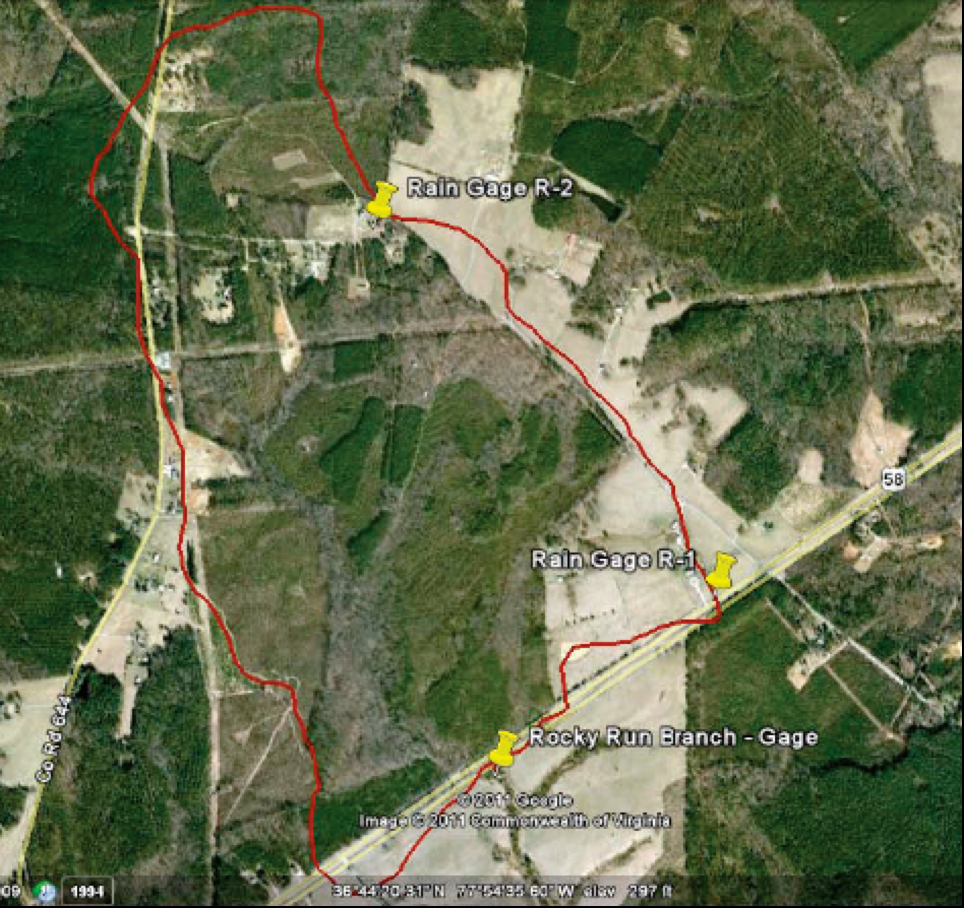
\includegraphics[width=5.0in]{RockyRun.jpg} 
   \caption{Rocky Run Branch Watershed}
   \label{fig:RockyRun}
\end{figure}
\begin{enumerate}
\item Estimate the time of concentration using the Kerby-Kirpich method assuming the slope is 0.006 along the main channel (which drains to the outlet).  The channel is clearly visible at the gage and running northward to the utility easement about 2/3 up the watershed.  Beyond the easement use your judgment as to the channel alignment. 
\item Estimate the time of concentration using the NRCS-Upland method assuming the slope is 0.006 along the main channel (which drains to the outlet).  The channel is clearly visible at the gage and running northward to the utility easement about 2/3 up the watershed.  Beyond the easement use your judgment as to the channel alignment. 
\item Research the readings and the internet and select an additional (different) method to estimate the time of concentration -- compare the three estimates and select the estimate you would choose and explain why you would make that choice.

\item Assume the utility easment is a barrier to overland flow, and runoff can only cross at a culvert as depicted in Figure \ref{fig:RockyRunSubDivide}. The easement divides the watershed into two smaller watersheds; the upper watershed whose outlet is the culvert, and the lower watershed with same outlet as before.

\begin{figure}[h!] %  figure placement: here, top, bottom, or page
   \centering
   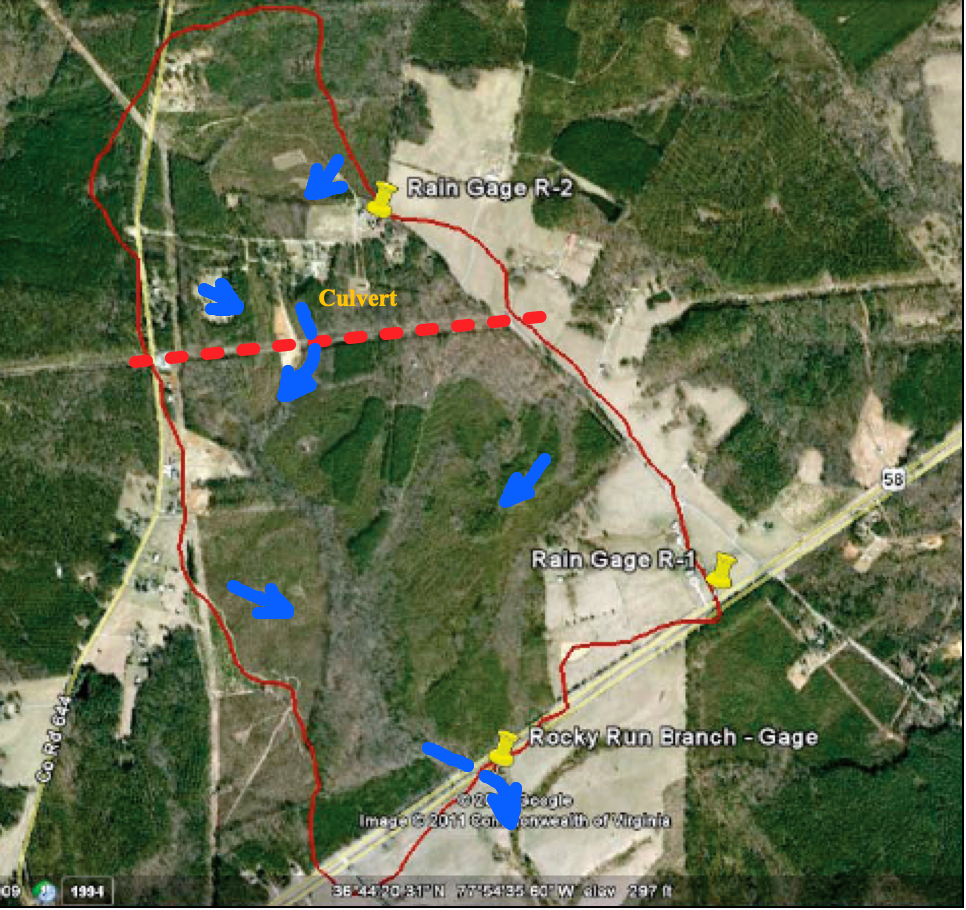
\includegraphics[width=5.0in]{RockyRunSubDivide.jpg} 
   \caption{Rocky Run Branch Watershed - Utility Easement as Barrier}
   \label{fig:RockyRunSubDivide}
\end{figure}

Estimate the time of concentration(s) using the three methods in both the upper and lower watershed.\footnote{The SCS Reservoirs in the Hardin Creek project behave similarly in that they divide the watershed into several parts which behave independently with regards to $T_C$.}

%\item Estimate the watershed runoff depth using the SCS CN model for a 5-year design rainfall.  Describe how you determined the land cover conditions to select an appropriate curve number.
\end{enumerate}


%\item Blaney-Criddle San Angelo
%\item Thornwaithe San Angelo
%\item CN Concho
%\item Green-Ampt concho


\end{document}  